\documentclass{beamer}
\usepackage{amsfonts,amsmath,oldgerm}
\usetheme{sintef}
\usepackage{xeCJK}
\usepackage{geometry}
\usepackage{fontspec}
\usepackage{hyperref}
\usepackage{bbm}
\usepackage{amsthm}

\geometry{paperwidth=16cm, paperheight=9.45cm}

\setCJKmainfont{STKaiti}

\newcommand{\testcolor}[1]{\colorbox{#1}{\textcolor{#1}{test}}~\texttt{#1}}

\titlebackground*{assets/background}

\newcommand{\hrefcol}[2]{\textcolor{cyan}{\href{#1}{#2}}}

\title{Machine Learning}
\subtitle{2024 Fall, Final Review}
% \course{Master's Degree in Computer Science}
\author{Xiangchen Tian}
\date{Jan 2, 2025}

\begin{document}
\maketitle

\section{SVM}

\begin{frame}{Support Vector Machine(a.k.a. SVM)}

\begin{itemize}
    \item 支持向量机是一种监督学习算法
    \item 通过构造极大边距超平面以更好泛化
    \item 两种常见形式:Hard-SVM 和 Soft-SVM
\end{itemize}
\end{frame}

\begin{frame}[fragile]{Hard-SVM}
    \begin{itemize}
        \item 设训练数据集 $S=\left\{ (\mathbf x_1, y_1), (\mathbf x_2, y_2), \cdots, (\mathbf x_m, y_m) \right\} $ ,其中$\mathbf x_i \in \mathbb R^d$,$y_i \in \left\{ -1, 1 \right\} $。
        \item 线性可分数据集:存在一个超平面 $(\mathbf w, b)$ 使 $\forall i, y_i = \text{sign}(\left\langle \mathbf w , \mathbf x_i \right\rangle +b )$。
        \item Hard-SVM 只能处理线性可分数据集。
    \end{itemize}
    算法:
    \begin{center}
        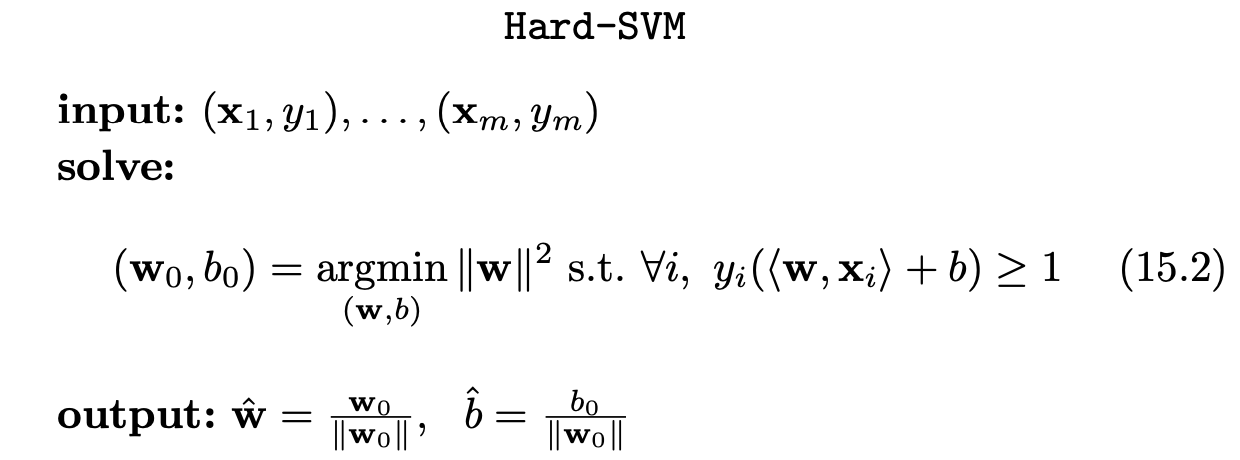
\includegraphics[width=0.6\textwidth]{assets/hsvm.png}
    \end{center}
    分析:固定标度最大化边距,相当于固定边距最小化标度;最后归一化还原成固定标度最大化边距的结果。
    
\end{frame}

\begin{frame}[fragile]{Soft-SVM}
    \begin{itemize}
        \item Soft-SVM 可以处理非线性可分数据集。
        \item 思想:放宽限制为 $y_i (\left\langle \mathbf{w}, \mathbf{x}_i \right\rangle + b) \geqslant 1-\xi_i$
    \end{itemize}
    算法:
    \begin{center}
        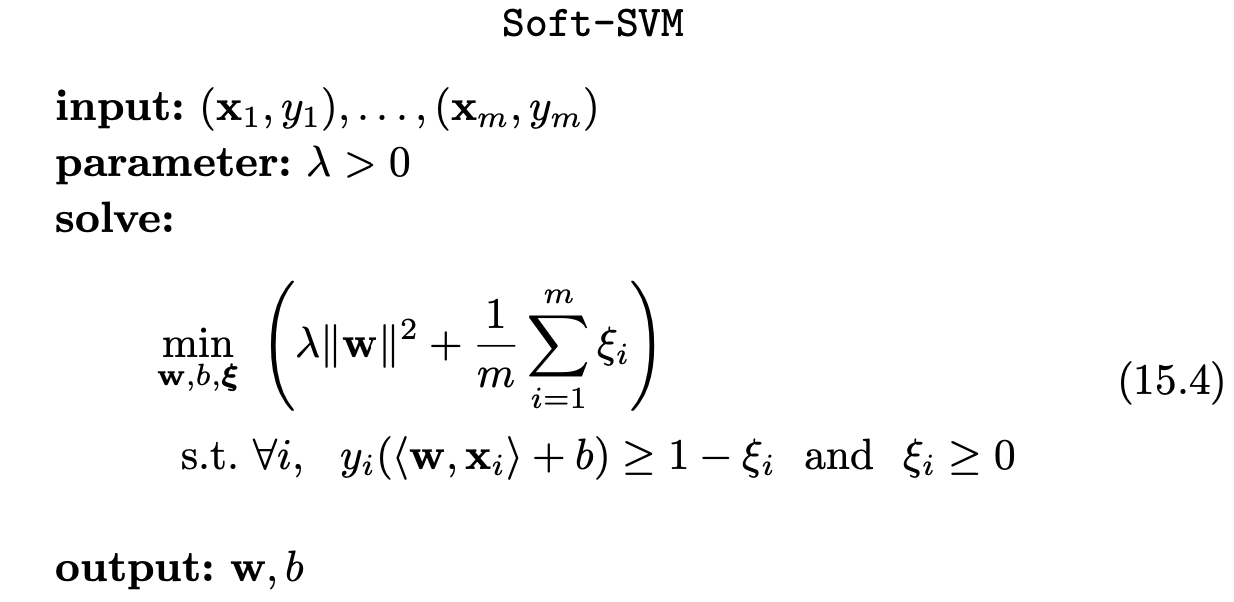
\includegraphics[width=0.6\textwidth]{assets/ssvm.png}
    \end{center}
    
\end{frame}

\begin{frame}[fragile]{hinge loss}
    \begin{itemize}
        \item 定义 hinge loss $\ell^{\text{hinge}}(x) =\max \left\{ 0, 1-x \right\}  $
        \item 定义 $L_S^{\text{hinge}}((\mathbf{w}, b)) = \frac{1}{m}\sum_{i=1}^{m} \ell^{\text{hinge}}(y_i\cdot(\left\langle \mathbf{w}, \mathbf{x}_i \right\rangle + b))$
        \item 注意到 (15.4) 式等价于
        \[
           \min_{\mathbf{w}, b} \left( \lambda \left\| \mathbf{w} \right\|^{2} + L_S^{\text{hinge}}((\mathbf{w}, b))  \right) 
        \]
        这就是标准的 regularized loss minimization problem,其中 $\lambda \left\| \mathbf{w} \right\|^{2}$ 是 $\ell_2$ 正则化。
        \item 因此 Soft-SVM 等价于一个hinge loss、$\ell_2$正则化的优化问题。
    \end{itemize}
\end{frame}

\begin{frame}[fragile]{duality}
    \begin{itemize}
        \item 以 Hard-SVM 为例(忽略$b$),定义
        \[
            g(\mathbf{w}) =\max_{\mathbf\alpha\in \mathbb{R}^{m},\mathbf \alpha \geqslant 0} \sum_{i=1}^{m} \alpha_i \cdot (1- y_i \cdot (\left\langle \mathbf{w}, \mathbf{x}_i \right\rangle)) = \begin{cases} 0 &\text{if }\forall i, y_i\left\langle \mathbf{w}, \mathbf{x}_i \right\rangle \geqslant 1   \\ +\infty & \text{otherwise} \end{cases}
        \]
        则(15.2) 式等价于
        \begin{align*}
            &\min_{\mathbf{w}} \left( \left\| \mathbf{w} \right\|^{2} + g(\mathbf{w})  \right)  \\
            = & \min_{\mathbf{w}} \max_{\mathbf\alpha\in \mathbb{R}^{m}, \mathbf\alpha \geqslant 0} \left( \left\| \mathbf{w} \right\|^{2} + \sum_{i=1}^{m} \alpha_i \cdot (1- y_i \cdot (\left\langle \mathbf{w}, \mathbf{x}_i \right\rangle))  \right) = p^{*} \\
            \geqslant & \max_{\mathbf\alpha\in \mathbb{R}^{m}, \mathbf\alpha \geqslant 0} \min_{\mathbf{w}} \left( \left\| \mathbf{w} \right\|^{2} + \sum_{i=1}^{m} \alpha_i \cdot (1- y_i \cdot (\left\langle \mathbf{w}, \mathbf{x}_i \right\rangle))  \right) = d^{*} \tag{1}
        \end{align*}

        \item 在Hard-SVM中,由于特殊条件的满足,$p^{*} = d^{*}$,所以可以通过求解对偶问题来求解原问题。
    \end{itemize}
\end{frame}

\begin{frame}[fragile]{duality}
    \begin{itemize}
        \item 对内部 $\mathbf{w}$ 取最小值,得到 $\mathbf{w} = \sum_{i=1}^{m} \alpha_i y_i \mathbf{x}_i$
        \item 带回对偶问题$(1)$式,得到 
        \[
            \max_{\mathbf\alpha\in \mathbb{R}^{m}, \mathbf\alpha \geqslant 0} \left( \sum_{i=1}^{m} \alpha_i - \frac{1}{2} \sum_{i=1}^{m} \sum_{j=1}^{m} \alpha_i \alpha_j y_i y_j \left\langle \mathbf{x}_i, \mathbf{x}_j \right\rangle  \right)
        \]
        \item 关键:只与 $\left\langle \mathbf{x}_i, \mathbf{x}_j \right\rangle$ 有关,而不与 $\mathbf{x}_i$ 有关,这是核技巧的基础。
    \end{itemize}
\end{frame}

\begin{frame}[fragile]{kernel method}
    \begin{itemize}
        \item 思想:由于很多问题在原空间中线形不可分,希望先将原数据点映射到一个(更高维)空间中,然后在更高维空间中执行SVM算法。
        \item 算法:
        \begin{itemize}
            \item 设原数据点定义域为$X$, 映射函数为 $\phi: X \to F$,其中 $F$ 是特征空间(feature space)。
            \item 给定原带标签数据集 $S=\left\{ (\mathbf x_1, y_1), (\mathbf x_2, y_2), \cdots, (\mathbf x_m, y_m) \right\} $,构造像数据集 $\hat S = \left\{ (\phi(\mathbf x_1), y_1), (\phi(\mathbf x_2), y_2), \cdots, (\phi(\mathbf x_m), y_m) \right\} $。
            \item 在$\hat S$上执行SVM算法,得到超平面 $(\mathbf w, b)$,对应一个线性分类器$h: \psi(\mathbf{x}) \mapsto y$。
            \item 预测原空间中test set example $\mathbf{x}$ 为 $h(\psi(\mathbf{x}))$
        \end{itemize}
    \end{itemize}
\end{frame}

\begin{frame}[fragile]{kernel}
    \begin{itemize}
        \item kernel 是 feature space 中的 inner product。
        \item 给定 embedding $\phi: X \mapsto F$, 定义 kernel function 
        \[
            K(\mathbf{x}, \mathbf{x'}) = \left\langle \phi(\mathbf{x}), \phi(\mathbf{x'}) \right\rangle
        \]
        \item $K$ 表征了$\mathbf{x}, \mathbf{x'}$ 的相似度
    \end{itemize}
\end{frame}

\begin{frame}[fragile]{kernel trick}
    \begin{itemize}
        \item 很多SVM问题都可以总结为以下 general 问题的实例:
        \[
           \min_{\mathbf{w}} \left( f(\left\langle \mathbf{w}, \mathbf{x}_1 \right\rangle, \left\langle \mathbf{w}, \mathbf{x}_2 \right\rangle, \cdots, \left\langle \mathbf{w}, \mathbf{x}_m \right\rangle ) + R(\left\| \mathbf{w} \right\|_2 )\right) 
        \]
        \item Example 1: Soft-SVM, $R(a) = \lambda a^{2}$, $f(a_1, a_2, \cdots, a_m) = \frac{1}{m} \sum_{i=1}^{m}\max \left\{ 0, 1-y_i a_i \right\} $
        \item Example 2: Hard-SVM, $R(a) = a^{2}$, $f(a_1, a_2, \cdots, a_m) = \begin{cases} 0 & \text{if } \exists  b \text{ s.t. } y_i (a_i+b) \geqslant 1 \\ +\infty & \text{otherwise} \end{cases} $
        \item 而 $\mathbf{w} \in \text{span}(\mathbf{x}_1, \mathbf{x}_2, \cdots, \mathbf{x}_m)$(\href{https://www.cs.huji.ac.il/w~shais/UnderstandingMachineLearning/understanding-machine-learning-theory-algorithms.pdf}{\underline{reference}}, Theorem 16.1), 因而事实上不会涉及 $\mathbf{x}_i$ 的具体值,只会涉及到 $\left\langle \mathbf{x}_i, \mathbf{x}_j \right\rangle$。
        \item 因此,只需要知道 kernel function $K(\mathbf{x}_i, \mathbf{x}_j)$,就能隐式在高维特征空间中执行SVM算法。
    \end{itemize}
\end{frame}

\begin{frame}[fragile]{characterizing kernel function}
    \begin{itemize}
        \item 一个良定义的 kernel function 必须对应一个合理的feature space embedding $\phi$。自然的问题:什么样的 kernel function 是合理的?
        \begin{block}{Mercer's Theorem}
            一个对称函数 $K:X\times X \to \mathbb{R}$ (对称:$K(\mathbf{x}, \mathbf{x'}) = K(\mathbf{x'}, \mathbf{x}), \forall \mathbf{x}, \mathbf{x'} \in X$)可实现为某特征空间中的内积,当且仅当$K$对应的 Gram matrix 是半正定的。
        \end{block}
        \item Gram matrix $G: G_{ij} = K(\mathbf{x}_i, \mathbf{x}_j)$.
        \item 证明思路:($\Rightarrow $)straight forward,($\Leftarrow $)采用构造法,构造出一个特征空间和一个内积,使得这个内积对应的 kernel function 为 $K$。
    \end{itemize}

\end{frame}

\section{Decision Trees}

\begin{frame}{Decision Trees}
\begin{block}{Decision Tree}
    一个决策树是一个 Boolean Function $f: \mathbb{F}_2^{n} \to \mathbb{R}$ 的表示方法。它是一个含根二叉树,其中内部节点由某个$i \in [n]$来标记,每个内部节点的出边被标记为$0$或$1$,每个叶子节点都有一个实数值,且要求没有$i \in [n]$在一条从根到叶节点的路径上出现多于一次。
\end{block}
\begin{itemize}
    % \item 决策树是一个预测器$h: X \to Y$, 方法是从树的根节点一次访问每个孩子节点判断下一步走向,最终走到叶子节点。每个叶子节点对应一个$Y$中的元素。
    \item 称决策树的叶节点总个数为决策树的大小(size) $s$,称决策树根到叶节点路径的最大长度为决策树的深度(depth) $d$。
    \item 根据定义,每个决策树都对应一个有$n$个变量的布尔函数。
\end{itemize}
\end{frame}

\begin{frame}{Decision Trees Example}
    Example:
    \begin{center}
        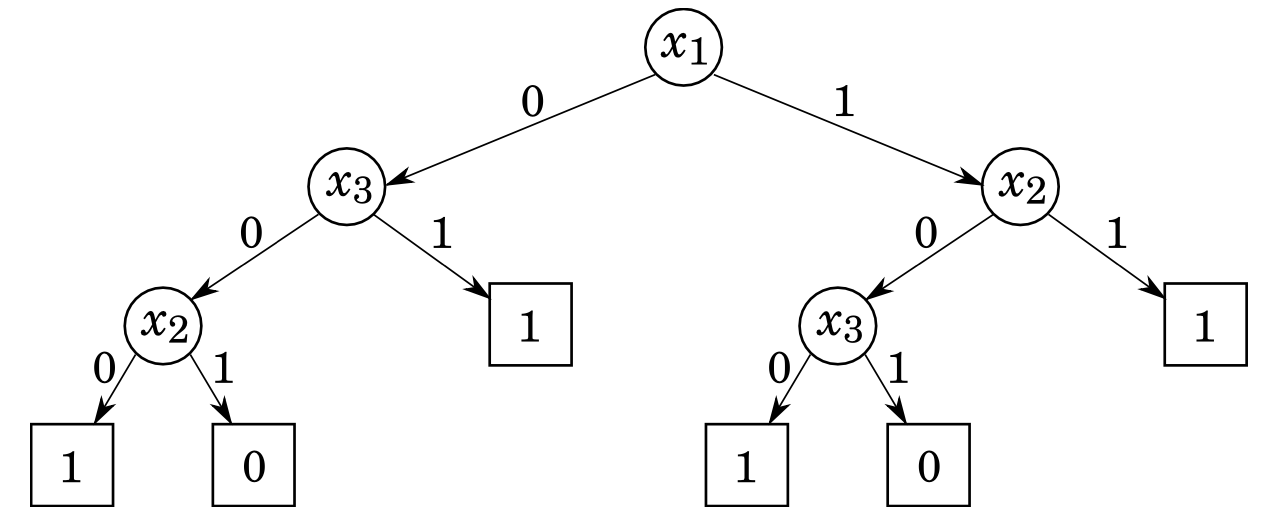
\includegraphics[width=0.65\textwidth]{assets/dtree.png}
    \end{center}

    Note: 这棵树事实上对应函数 $\text{Sort}_3$, 其中 $\text{Sort}_3(x_1, x_2, x_3) = 1$ 当且仅当 $x_1 \geqslant x_2 \geqslant x_3$ 或 $x_1 \leqslant x_2 \leqslant x_3$。
\end{frame}

\begin{frame}{Theoretical Guarantee}
    \begin{block}{Theorem: Convert decision tree to low degree sparse function}
        对任意有$s$个叶节点的决策树$T$,存在一个degree为$\log(s / \epsilon)$,$L_0$-norm(sparsity) 为 $s^{2} / \epsilon$ 的布尔函数 $h$ 能够 $4 \epsilon$-approximate $T$。 
    \end{block}
    证明思路:
    \begin{itemize}
        \item 将决策树$T$截断到深度为 $\log(s / \epsilon)$,最大误差为$\epsilon$。
        \item 截断后的树$T'$ 能用一个$L_1(f) \leqslant s, \text{deg}(f) = \log(s / \epsilon)$的布尔函数$f$ 严格表示。
        \item 上述满足$L_1(f) \leqslant s, \text{deg}(f) = \log(s / \epsilon)$的布尔函数$f$能用另一个满足$L_0(h) \leqslant s^{2} / \epsilon, \text{deg}(h) = \log (s / \epsilon)$的布尔函数$h$ 来 $\epsilon$-approximate 表示。
    \end{itemize}
    综上,$\left\| T-f \right\|^{2} \leqslant \epsilon$, $\left\| f-h \right\|^{2} \leqslant \epsilon$ 
    
    $\implies \left\| T - h \right\|^{2} \leqslant 2 \left\| T-f \right\|^{2} + 2 \left\| f-h \right\|^{2} \leqslant 4\epsilon$
\end{frame}

\begin{frame}{Practical Algorithms 1}
    由于使用上述定理提供的方法求low degree approximate function $h$要求已知决策树内部结构,但实际中决策树是黑箱,只能通过多次输入查看输出得到决策树的信息。实际中采用以下几种采样算法:
    \begin{itemize}
        \item LMN: 设$T$对应布尔函数$f$,均匀采样$m$个$f$ 定义域内的点$\left\{ x_i, i \in [m] \right\} $,计算 $f(x_i)$,对每个$|S| \leqslant \log(s / \epsilon)$的 $S$ 估计傅立叶系数$\hat{f}(S)\approx \frac{1}{m} \sum_{i=1}^{m} f(x_i) \chi _S(x_i)$。
        最后返回
        \[
            h = \sum_{S: |S| \leqslant \log(s / \epsilon)} \hat{f}(S) \chi _S
        \]
        \item Harmonica: 这个问题本质上是求一个在傅立叶基下稀疏的布尔函数,可以用compress sensing 范式求解。
    \end{itemize}
    \begin{center}
        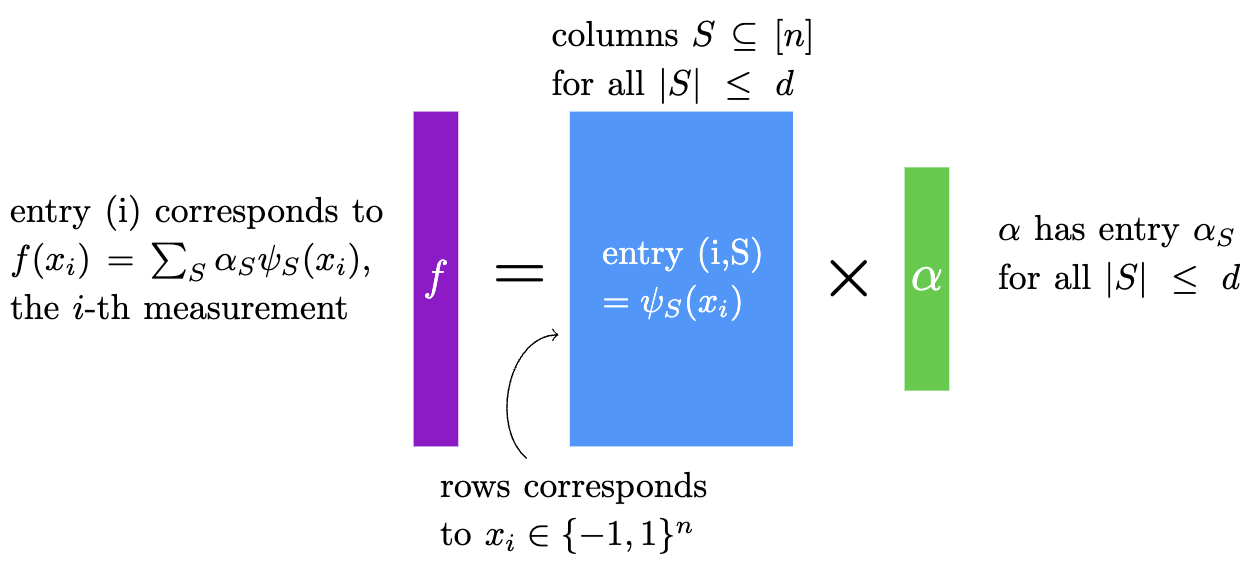
\includegraphics[width=0.4\textwidth]{assets/harmonica.png}
    \end{center}

\end{frame}

\begin{frame}{Practical Algorithms 2}
    现实问题中的决策树:给定若干样例,希望从样例中学习决策树。

    Example:
    \begin{center}
        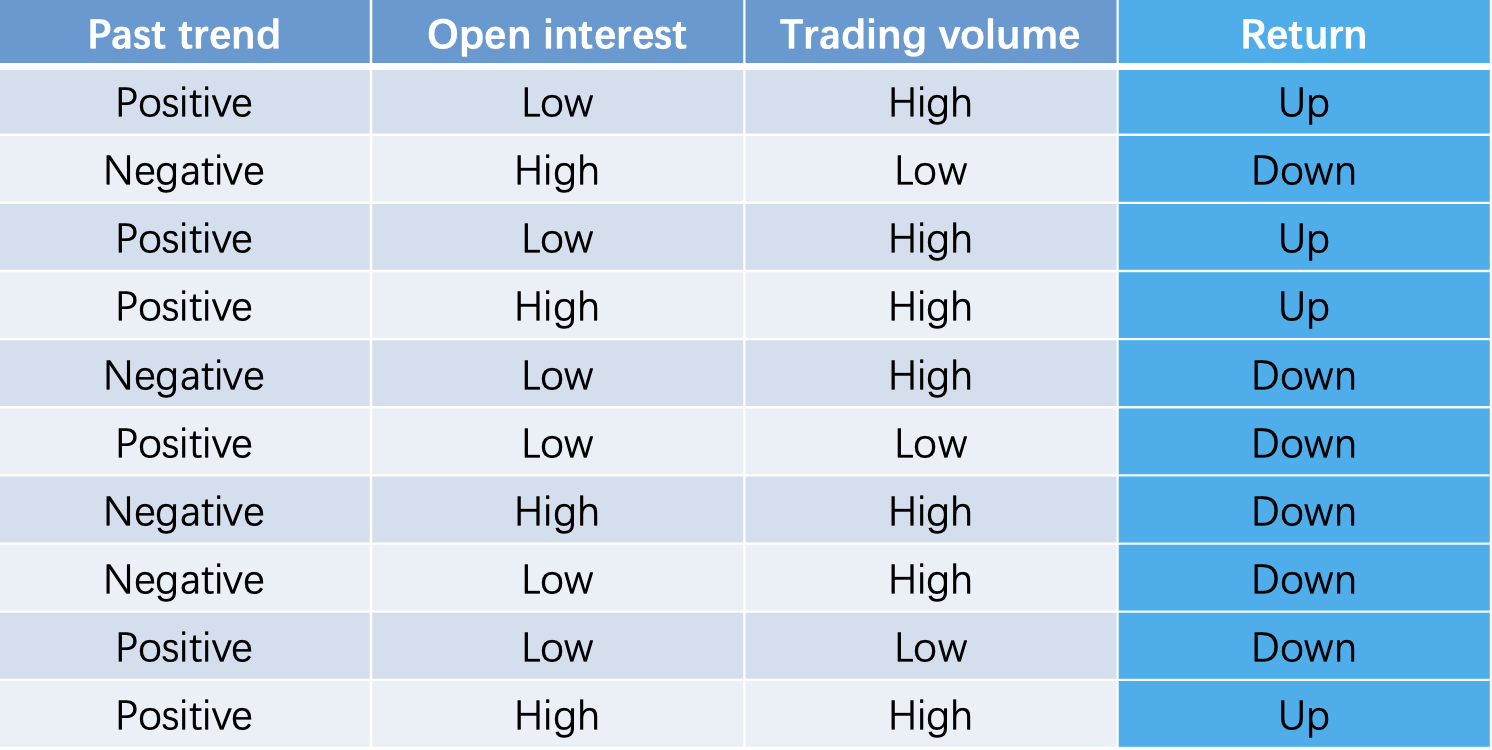
\includegraphics[width=0.65\textwidth]{assets/learndte.png}
    \end{center}

\end{frame}

\begin{frame}{Practical Algorithms 2}
    与上面的approach不同,另一种方法是递归选取最重要的变量作为内部节点划分样例。

    算法:
    \begin{center}
        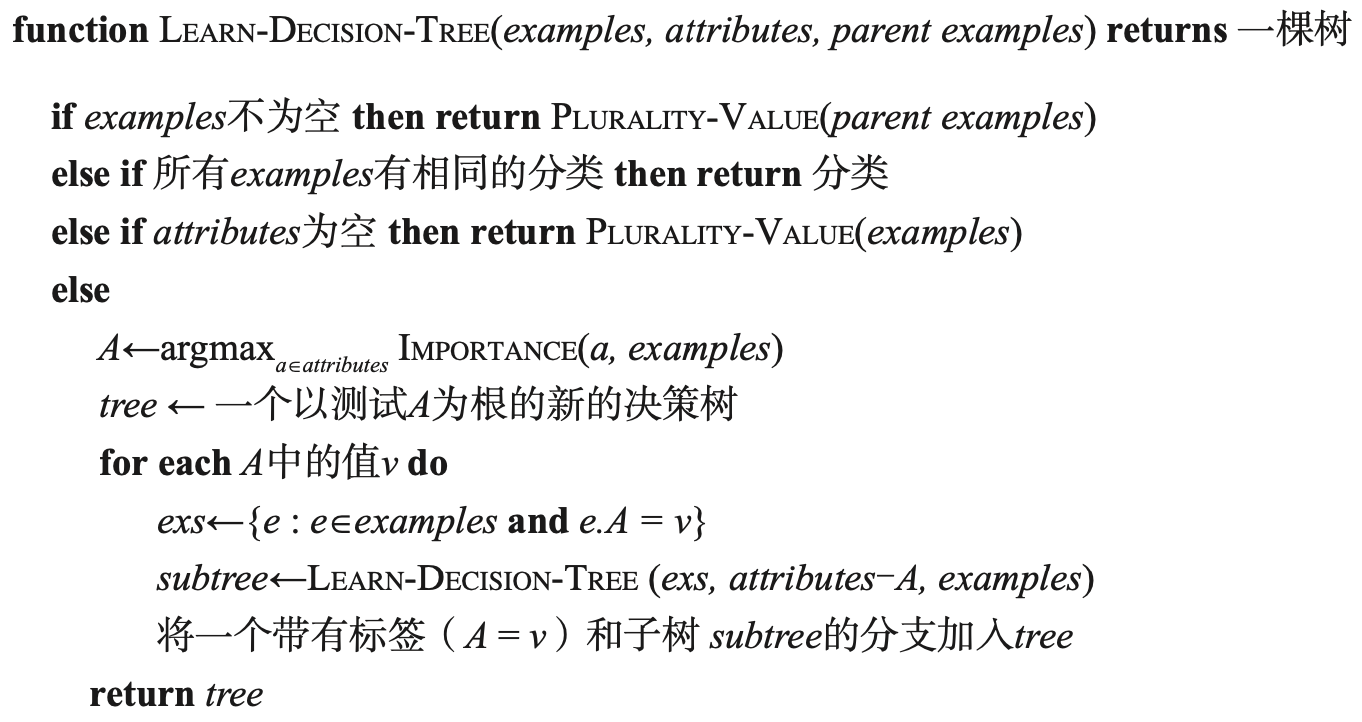
\includegraphics[width=0.6\textwidth]{assets/learndta.png}
    \end{center}
    解释:每次根据某种准则选择最重要的变量$i$(若某变量的取值几乎决定了最终的类别是什么,说明这个变量较重要)

\end{frame}

\begin{frame}{Gini Index}
    \begin{itemize}
        \item Gini Index 是一种判断某个变量是否重要的一种准则。
        \item 定义:对变量A,$\text{Gini}(A)= \sum_{a} p(A=a) \text{Gini}(a)$, 其中$\text{Gini}(a) = 1- \sum_{i}p_i^{2}$(详见课件例子)
        \item $\text{Gini}(a)$ 越小表示区分度越好(如果一个变量$A$取正时所有结果都是正,一个变量取负时所有结果都是负,则$\text{Gini}(A) = 0$),故每次划分变量时选择$\text{Gini}(A)$最小的变量$A$。
        \item 其他准则:Information Gain
    \end{itemize}
\end{frame}

\section{Boosting}

\begin{frame}{Boosting}

\begin{itemize}
    \item 思想:希望能有一种方法能够聚合多个弱学习器(每个弱学习器可以只比随机猜测表现好一点),使得整体学习器的性能更好。
    \item 一次性学习强学习器可能计算复杂度上承担不起,但每个弱学习器的计算复杂度较低,聚合多个弱学习器的计算复杂度可以接受。
\end{itemize}
\end{frame}

\begin{frame}{AdaBoost (a.k.a Adaptive Boosting)}
\begin{itemize}
    \item AdaBoost是最典型的boosting算法。
    \item AdaBoost 思想:在简单假设类上构建线性预测期作为更强大的假设类。
\end{itemize}
算法:
\begin{center}
    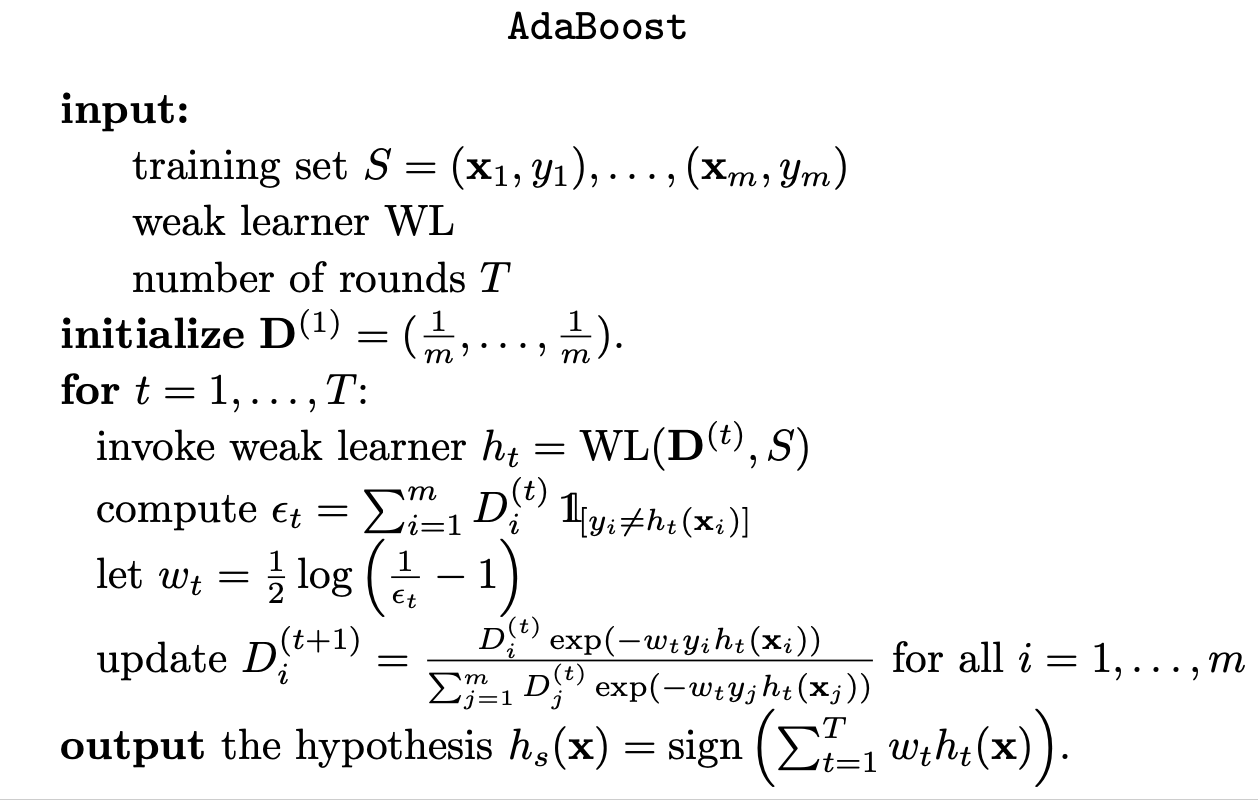
\includegraphics[width=0.6\textwidth]{assets/adaboost.png}
\end{center}
\end{frame}

\begin{frame}{AdaBoost Analysis}
    \begin{block}{Theorem: AdaBoost Training Error Upper Bound}
        $S$ 是一个训练集,假设在 AdaBoost 的每一次迭代中,弱分类器返回的假设满足 $\epsilon_t \leq \frac{1}{2} - \gamma$。则 AdaBoost 输出的最终假设的训练误差满足以下不等式:
        \[
        L_S(h_s) = \frac{1}{m} \sum_{i=1}^{m} \mathbbm{1}[h_s(x_i) \neq y_i] \leq \exp(-2 \gamma^2 T)
        \]
    \end{block}
    证明:
    对于每一轮 $t$,记 $f_t = \sum_{p<t} w_p h_p$,因此 AdaBoost 的输出为 $f_T$。此外,记
\[
Z_t = \sum_{i=1}^{m} \exp(-y_i f_t(x_i))
\]

\end{frame}

\begin{frame}{AdaBoost Analysis}
    注意到对于任何假设都有 $ \mathbbm{1}[h(x) \neq y] \leq \exp(-y h(x))$。因此,训练误差满足:
    \[
    L_S(f_T) \leq Z_T
    \]
    所以我们只需证明 $Z_T \leq \exp(-2 \gamma^2 T)$。为了bound 住 $Z_T$,我们将其重写为:
    \[
    Z_T =  \frac{Z_T}{Z_{T-1}} \cdot \frac{Z_{T-1}}{Z_{T-2}}  \cdots \frac{Z_2}{Z_1} \cdot \frac{Z_1}{Z_0}
    \]
    其中我们使用了 $Z_0 = 1$,因为 $f_0 \equiv 0$。现在我们只需证明对于每一轮 $t$:
    \[
    \frac{Z_{t+1}}{Z_t} \leq \exp(-2 \gamma^2)
    \]
    为了证明上式,首先通过简单的归纳推理可知对于所有的 $t$ 和 $i$都有:
    \[
    D_{i}^{(t+1)} = \frac{\exp(-y_i f_t(x_i))}{\sum_{j=1}^{m} \exp(-y_j f_t(x_j))}
    \]
\end{frame}

\begin{frame}{AdaBoost Analysis}
    因此:
    \[
    \frac{Z_{t+1}}{Z_t} = \frac{\sum_{i=1}^{m} \exp(-y_i f_{t+1}(x_i))}{\sum_{j=1}^{m} \exp(-y_j f_t(x_j))} = \frac{\sum_{i=1}^{m} \exp(-y_i f_t(x_i)) \exp(-y_i w_{t+1} h_{t+1}(x_i))}{\sum_{j=1}^{m} \exp(-y_j f_t(x_j))}
    \]
    \[
    \implies \frac{Z_{t+1}}{Z_t} = \exp(-w_{t+1}) \left(1 - \epsilon_{t+1}\right) + \exp(w_{t+1}) \epsilon_{t+1} = 2 \sqrt{\epsilon_{t+1}(1 - \epsilon_{t+1})}
    \]
    根据我们的假设,$\epsilon_{t+1} \leq \frac{1}{2} - \gamma$。由于函数 $g(a) = a(1 - a)$ 在区间 $[0, \frac{1}{2}]$ 上是单调递增的,我们得到:
    \[
    2 \sqrt{\epsilon_{t+1}(1 - \epsilon_{t+1})} \leqslant 2 \sqrt{\left(\frac{1}{2} - \gamma\right) \left(\frac{1}{2} + \gamma\right)} \leqslant \sqrt{1 - 4 \gamma^2} 
    \]
    因此,$\frac{Z_{t+1}}{Z_t} \leq \exp(-2 \gamma^2)$。\qed
\end{frame}
\section{PCA}

\begin{frame}{Principal Component Analysis (a.k.a. PCA)}
\begin{itemize}
    \item PCA是一种降维技术,将高维空间中的数据映射到低维空间。
    \item 详细请参考计算机与人工智能应用数学
    \item power method:一种高效求解最大本征值和对应的本征向量的方法
\end{itemize}
\end{frame}
\section{Nearest Neighbor and LSH}

\begin{frame}{Nearest Neighbor}
\begin{itemize}
    \item Nearest Neighbor 是一种非参数化模型。(数据集就是参数)
    \item 直接用遍历所有点的方式找到邻居的方法非常耗时,希望有一种数据结构能够高效返回近似最近邻
    \item LSH algorithm
\end{itemize}
\end{frame}

\begin{frame}{LSH}
    
\end{frame}
\section{Metric Learning}

\begin{frame}{Metric Learning}
    \begin{itemize}
        \item 核心思路:用neural network 训练出一个good feature space, 在此空间中有更好的nearest neighbor structure.
        \item Example: 图片分类问题中旋转物体视角、改变颜色、图片伸缩裁剪可能不会改变类别,但在像素空间中这些点相距非常远。
        \item 两种算法:NCA, LMNN
    \end{itemize}
    
\end{frame}

\begin{frame}{NCA}
    \begin{itemize}
        \item 希望学习一个函数$f$从原空间映射到有良好最近邻结构的feature space.
        \item 定义原空间中两点$x_i, x_j$的相似度为:
        \[
        p_{ij} = \frac{\exp(-\|f(x_i) - f(x_j)\|^2)}{\sum_{k \neq i} \exp(-\|f(x_i) - f(x_k)\|^2)}, i \neq j
        \]
        \[
            p_{ii} = 0
        \]
        \item 记$C_i = \left\{ j | c_i = c_j \right\} $为与$i$有相同label的下标集合,$P_i = \sum_{j\in C_i} p_{ij}$ 为$x_i$ 与其他与$x_i$有相同label的元素的总相似度。
        \item Loss function: $L(A) = \sum_{i} P_i$,用于训练$f$模型中的参数。
    \end{itemize}
\end{frame}

\begin{frame}{LMNN}
    \begin{itemize}
        \item TODO
    \end{itemize}
\end{frame}
\section{Clustering}

\begin{frame}{Clustering}
    Clustering 任务:输入元素集合$X$及一个距离函数$d: X\times X \to  \mathbb{R}_+$(满足$d(x, y) = d(y, x)$ 和 $d(x, x) = 0$, $\forall x, y \in X$), ,Cluster算法应该输出一个划分 (partition) $C = \left\{ C_1, C_2, \ldots, C_k \right\}$,其中$C_i \subseteq X$,且$\bigcup_{i=1}^{k} C_i = X$。
    典型算法:
    \begin{itemize}
        \item Linkage-based clustering
        \item K-means
        \item Spectral clustering
    \end{itemize}
\end{frame}

\begin{frame}{K-means: Lloyd's method}
    算法:
    \begin{center}
        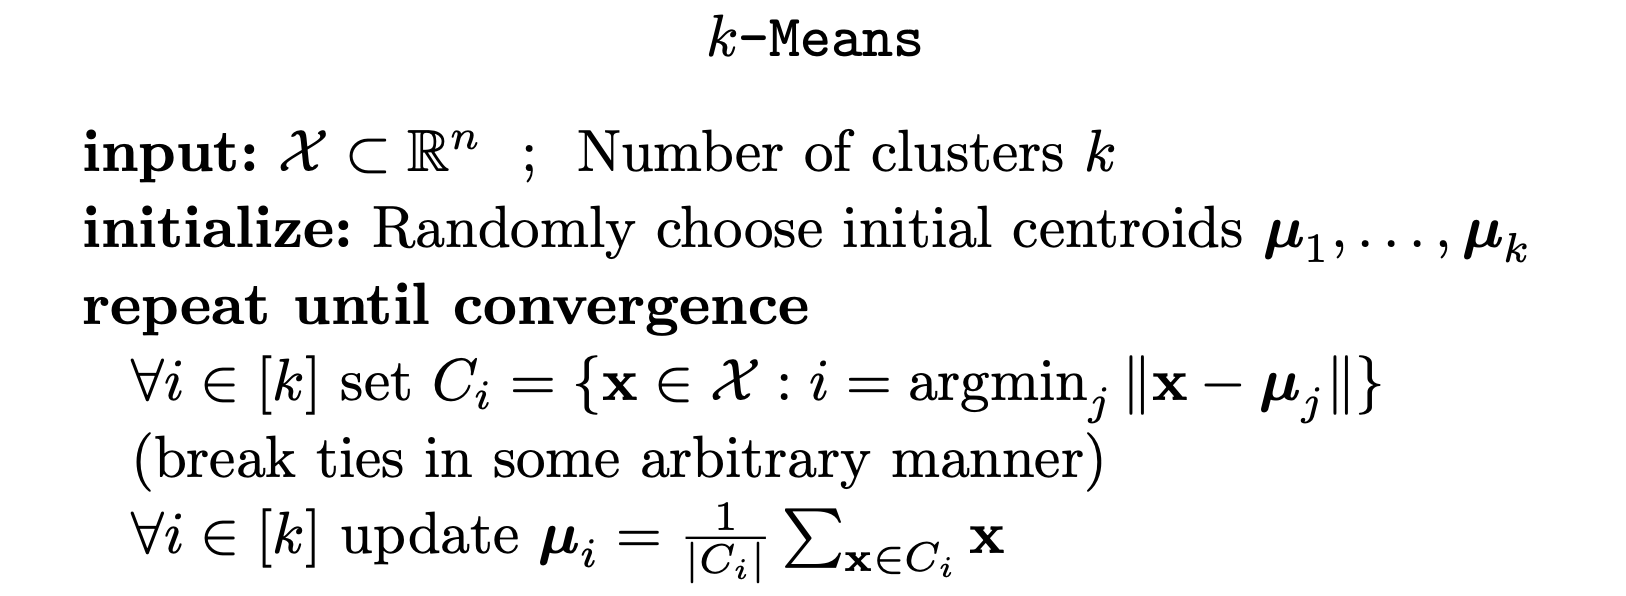
\includegraphics[width=0.65\textwidth]{assets/kmeans.png}
    \end{center}
    Example: 参考上课slides。
\end{frame}

\begin{frame}{K-means: Lloyd's method}
\begin{itemize}
    \item 重要性质:每一次迭代过程中,objective function 
    \[
        G_{\text{K-means}}((X, d), (C_1, C_2, \cdots, C_k)) =\min_{\mu_1, \mu_2, \cdots, \mu_k} \sum_{i=1}^{k} \sum_{x \in C_i} d(x, \mu_i) ^{2}
    \]
    不会增加。
    \item Note: Lloyd's method是最常用的一种K-means算法,但K-means算法还有很多其他变种。
\end{itemize}
\end{frame}

\begin{frame}{Spectral Clustering}
    \begin{itemize}
        \item 思想:用 similarity graph $G$ 表示集合 $X = \left\{ x_1, x_2, \cdots, x_m \right\}$各点之间的关系。$G=(V, E)$,其中$V=\left\{ x_1, x_2, \cdots, x_m \right\} $, 每两个顶点之间连接一条权重为$W_{ij} = s(x_i, x_j)$的边,$s$是相似度度量,例如$s(x_i, x_j) = \exp\left( \frac{d(x_i, x_j)^{2}}{\sigma^{2}} \right) $
        \item Clustering问题可表述为:希望找到一种partition,同一part各点之间边权重较大,不同part各点之间边权重较小。
        \item 最小化 $Cut(C_1, C_2, \cdots, C_k) = \sum_{i=1}^{k} \sum_{r \in C_i, s \notin C_i} W_{rs}$ 经常会将单独一个点作为一个part。
        \item 解决办法:最小化 $RatioCut(C_1, C_2, \cdots, C_k) = \sum_{i=1}^{k} \frac{\sum_{r \in C_i, s \notin C_i} W_{rs}}{|C_i|}$,权衡part大小和part间边权重。
    \end{itemize}
\end{frame}

\begin{frame}{Spectral Clustering Analysis}
    \begin{block}{Definition: Unnormalized Graph Laplacian}
        一个有向图的unnormalized graph Laplacian定义为$L = D - W$,其中$D$是degree matrix,$D_{ii} = \sum_{j=1}^{m} W_{ij}$,$W$是边权重矩阵,对角元均为$0$。
    \end{block}
    \begin{block}{Lemma}
        设 $C = \left\{ C_1, C_2, \cdots, C_k \right\} $是一个clustering,定义$H \in \mathbb{R}^{m\times k}$:
        \[
            H_{ij} = \frac{1}{\sqrt{|C_j|}} \mathbbm 1[i \in C_j]
        \]
        则 $H^{T}H = I^{k\times k}$且$\text{RatioCut}(C_1, C_2, \cdots, C_k) = \text{tr}(H^{T}LH)$, 其中 $L$ 是similarity graph 的 unnormalized graph Laplacian.
    \end{block}
    证明思路:用$H$和$L$的定义直接得到。
\end{frame}

\begin{frame}{Spectral Clustering Analysis}
    根据上述Lemma,我们可以将RatioCut问题转化为如下问题:

    问题1 (original): 找一个矩阵$H \in \mathbb{R}^{m\times k}$,满足
    \begin{itemize}
        \item $H^{T}H = I$
        \item $H_{ij}=0$或$1/\sqrt{|C_j|}$
        \item 最小化 $\text{tr}(H^{T}LH)$
    \end{itemize}

    以上问题是一个integer programming problem,无法高效求解。所以对问题进行relax:

    问题2 (relax): 找一个矩阵$H \in \mathbb{R}^{m\times k}$,满足
    \begin{itemize}
        \item $H^{T}H = I$
        \item 最小化 $\text{tr}(H^{T}LH)$
    \end{itemize}
    这时问题变为标准的 PCA 问题,其解为$L$的对应前$k$个最小本征值的特征向量。
\end{frame}

\begin{frame}{Spectral Clustering Algorithm}
    算法:
    \begin{center}
        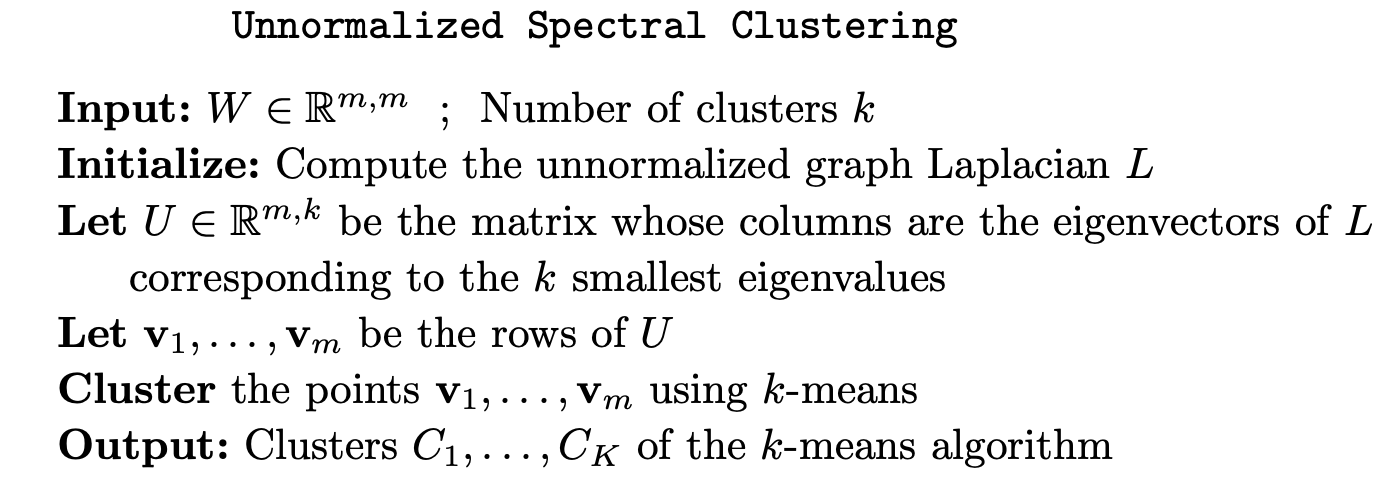
\includegraphics[width=0.7\textwidth]{assets/usc.png}
    \end{center}
\end{frame}

\begin{frame}{Birkhoff's Theorem}
    TODO
\end{frame}

\section{SimCLR}


\begin{frame}[fragile]{SimCLR}
    \begin{columns}
    \begin{column}{0.7\textwidth}
        \begin{itemize}
            \item Goal: 用 contrastive learning 方法学习图片的 visual representations。
            \item 训练集是若干无标签图像,希望对每个图像输出一个 feature vector。
        \end{itemize}
        右图中,$f$ 是一个神经网络,输入扰动后的图像,输出一个 feature vector。$g$ 是一个 projection head,将 feature vector 投影到一个用于衡量相似度的空间。
        
        $T$ 是对图像施加各种可能扰动的集合,例如随机裁剪、旋转、噪声、模糊等。
    \end{column}
    \begin{column}{0.3\textwidth}
        \begin{center}
            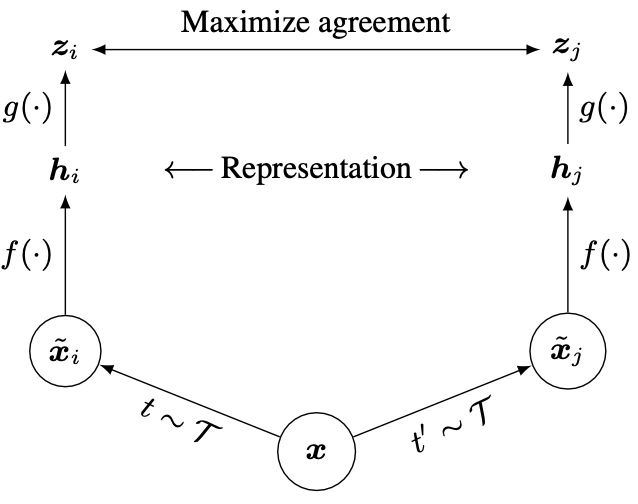
\includegraphics[width=\textwidth]{assets/simclr.png}
        \end{center}
    \end{column}
    \end{columns}
\end{frame}

\begin{frame}{SimCLR Algorithm}
    \begin{columns}
        \begin{column}{0.65\textwidth}
            \begin{itemize}
                \item Note: 其中 $\ell(i, j)$被称为 InfoNCE loss。
            \end{itemize}
        \end{column}
        \begin{column}{0.37\textwidth}
            算法:
            \begin{center}
                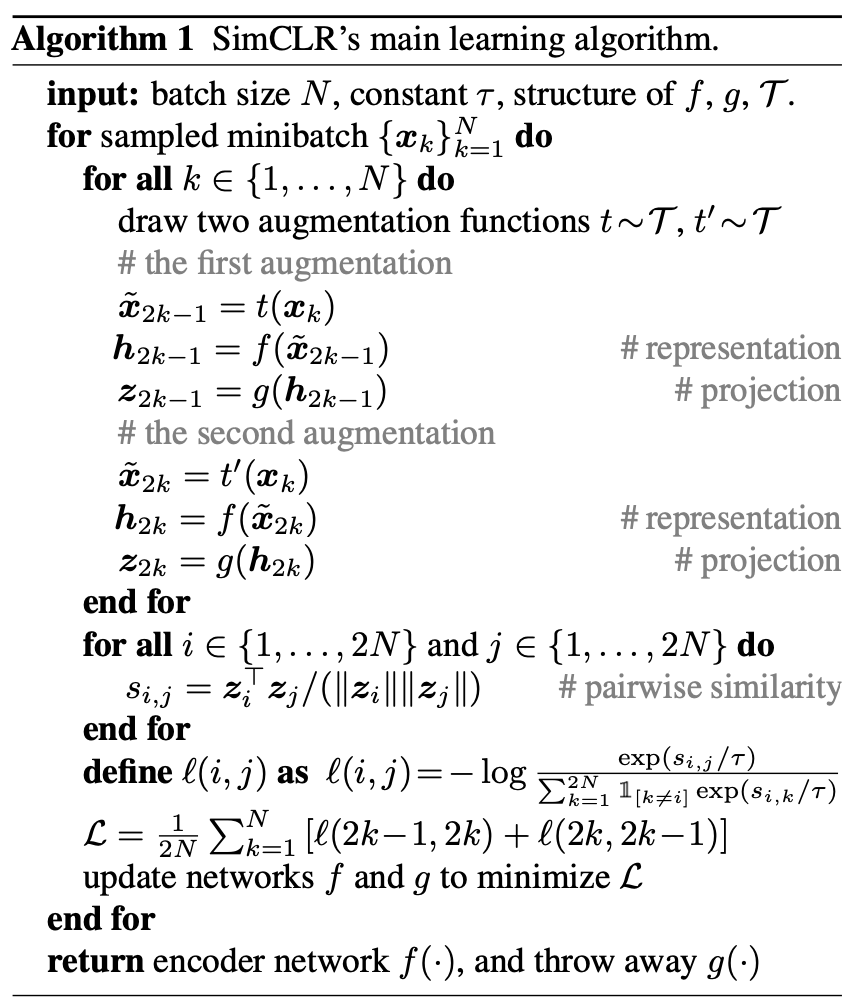
\includegraphics[width=\textwidth]{assets/simclra.png}
            \end{center}
                \end{column}
        \end{columns}
    
\end{frame}

\begin{frame}{Contrastive Learning is spectral clustering on similarity graph}
    Yang Yuan 组的一篇论文指出:
    \begin{itemize}
        \item 定义 Cross entropy loss $H_\pi^{k}(Z) = \mathbb{E}_{W_X\sim P(\cdot; \pi)} \left[ \log P(W_Z = W_X; K_Z) \right]$。
        \item 可以证明:Cross entropy loss 等价于 InfoNCE loss;
        \item Cross entropy loss 隐式在 similarity graph 上执行了 spectral clustering
        \item 所以 SimCLR 可以看作是 spectral clustering on similarity graph。
    \end{itemize}
    (把他课件上的内容差不多记住,作业那道题会做应该就行了)
\end{frame}

\begin{frame}{CLIP}
    \begin{itemize}
        \item CLIP 是一种多模态学习方法,可以同时处理图片和文本。
        \item 细节:给定一个batch of image-text pairs $(image, text)$数据,CLIP用一个 image encoder 和一个 text encoder 分别将 image 和 text 转换为 feature vectors对,然后用 InfoNCE 作为loss function 训练 encoder。
        \item CLIP 也隐式执行了 spectral clustering。
    \end{itemize}
\end{frame}

\section{t-SNE}

\begin{frame}{t-distributed Stochastic Neighbor Embedding (a.k.a. t-SNE)}
    t-SNE 是一种非线性降维算法,用于将高维数据 ($\left\{ x_1, x_2, \cdots, x_N \right\} $) 映射到低维空间 ($\left\{ y_1, y_2, \cdots, y_N \right\} $, 通常$y_i \in \mathbb{R}^{2}$ 或 $\mathbb{R}^{3}$, $i\in [N]$)。

    思想:t-SNE 分为两个阶段。
    \begin{itemize}
        \item 首先对每对高维对象分配一个概率,要求相似的对象有更高的概率,不相似的对象分配较低的概率。
        \item 然后,t-SNE 对低维空间定义一个类似的概率分布,并最小化与之前概率分布之间的 KL 散度。
    \end{itemize}
\end{frame}

\begin{frame}{SNE}
    \begin{itemize}
        \item SNE 是 t-SNE 的前身。
        \item 给定 $N$ 个高维空间对象的集合 $\left\{ x_1, x_2, \cdots, xN \right\} $, 定义
        \[
            p_{j|i} = \frac{\exp(-\|x_i - x_j\|^2 / 2\sigma_i^2)}{\sum_{k \neq i} \exp(-\|x_i - x_k\|^2 / 2\sigma_i^2)}, \forall i \neq  j
        \]
        \[
            p_{i|i} = 0
        \]
        显见 $ \sum_{j} p_{j|i} = 1$。
        \item 解释:按照高斯分布对所有$x_i$周围的点进行加权得到$x_j$对$x_i$的重要性。
        \item 定义 $p_{ij} = \frac{p_{j|i}+ p_{i|j}}{2N}$。
        \item $\sigma_i$ 的选取:用bisection method求解满足 $\text{perp}(P_i) = 2^{H(P_i)} = $预先人为设定值的 $\sigma_i$,其中$H(P_i) = - \sum_{j} p_{j|i} \log_2(p_{j|i})$。
        \item perplexity 可解释为一种平滑的邻居个数度量。$\text{perp}(P_i)$越大,$H(P_i)$越大,$p_{j|i}$分布越平均,$\sigma_i$越大,因此邻居越多。
    \end{itemize}
\end{frame}

\begin{frame}{SNE}
    \begin{itemize}
        \item 原始的SNE在低维空间也选取高斯分布进行距离度量。
        \[
            q_{ij} = \frac{\exp(-\|y_i - y_j\|^2)}{\sum_{k \neq i} \exp(-\|y_i - y_k\|^2)}, \forall i \neq  j
        \]
        其中$y_i$是$x_i$在低维空间中的对应点,$q_{ij}$是低维空间中相似度度量。
        \item 这存在 crowding problem。解释:``There are several reasons why the pairwise distances in a two-dimensional map cannot faithfully
        model distances between points on the ten-dimensional manifold.''
        \begin{itemize}
            \item 在10维空间中,可以有11个点彼此等距,但二维空间中无法忠实反映这种关系。
            \item 以数据点$x_i$为中心,半径为$r$的球体在10维空间中体积按照$r^{10}$缩放,因此,如果数据点在10维空间中$x_i$周围的区域中大致均匀分布,如果我们试图用相同的高斯分布对二维地图中$x_i$到其他数据点的距离进行建模,数据点会非常拥挤:二维空间中可用于容纳中等距离数据点的区域与可用于容纳附近数据点的区域相比远远不够大。
        \end{itemize}
    \end{itemize}
\end{frame}

\begin{frame}{t-SNE}
    \begin{itemize}
        \item 一种解决方案:``Mismatched Tails can Compensate for Mismatched Dimensionalities''
        \item 这就是t-SNE的思想:在高维空间中,使用 Gaussian Distribution 求数据点之间相似性;而在低维空间中,使用 Student t-distribution 求数据点之间相似性。
        \[
            q_{ij} = \frac{(1 + \|y_i - y_j\|^2)^{-1}}{\sum_{k \neq i} (1 + \|y_i - y_k\|^2)^{-1}}, \forall i \neq  j
        \]
        \item Student t-distribution 的尾部(正比于$\frac{1}{x^{2}}$)比高斯分布(正比于$\exp(-x^{2})$)更“重” ,因此等效于通过加重尾部概率分布缓解了 crowding problem。
        \item 最终训练的loss function:
        \[
            C = \text{KL}(P||Q) = \sum_{i\neq j} p_{ij} \log \frac{p_{ij}}{q_{ij}}
        \]
        \item 优化方法:求$\frac{\partial C}{\partial y_i}$更新 $y_i$在低维空间中的位置。
    \end{itemize}
\end{frame}


\section{Robust Machine Learning}

\begin{frame}{Robust Machine Learning}
    思想:很多机器学习算法只要对输入数据进行微小的扰动,输出结果就完全错误了。希望能有一种方法能够让机器学习算法对输入数据的扰动具有一定的鲁棒性。

    几种方法:
    \begin{itemize}
        \item FGSM: 当学习率趋于无穷时,先更新再投影到正方体内结果大概率是顶点上。
        \item PGD: run gradient descent, and then project it back.
    \end{itemize}
    
    详见 Yang Yuan slides。
\end{frame}

\begin{frame}{Robust Features are Important}
    \begin{itemize}
        \item 左图实验发现,从原始既包含Robust Features也包含Non-Robust Features的数据集上只提取Robust Features部分,并在获得的新数据集Robust dataset上进行训练,
        可以得到类似的standard accuracy和robust accuracy(与在原始训练集上训练的结果相比)。
        \item 这说明模型可以只从Robust Features中学习,而不必须学习Non-Robust Features。
        \item Note: Robust Features 通常指人能看到的特征,因为人识别就是Robust的。
    \end{itemize}
    \begin{center}
        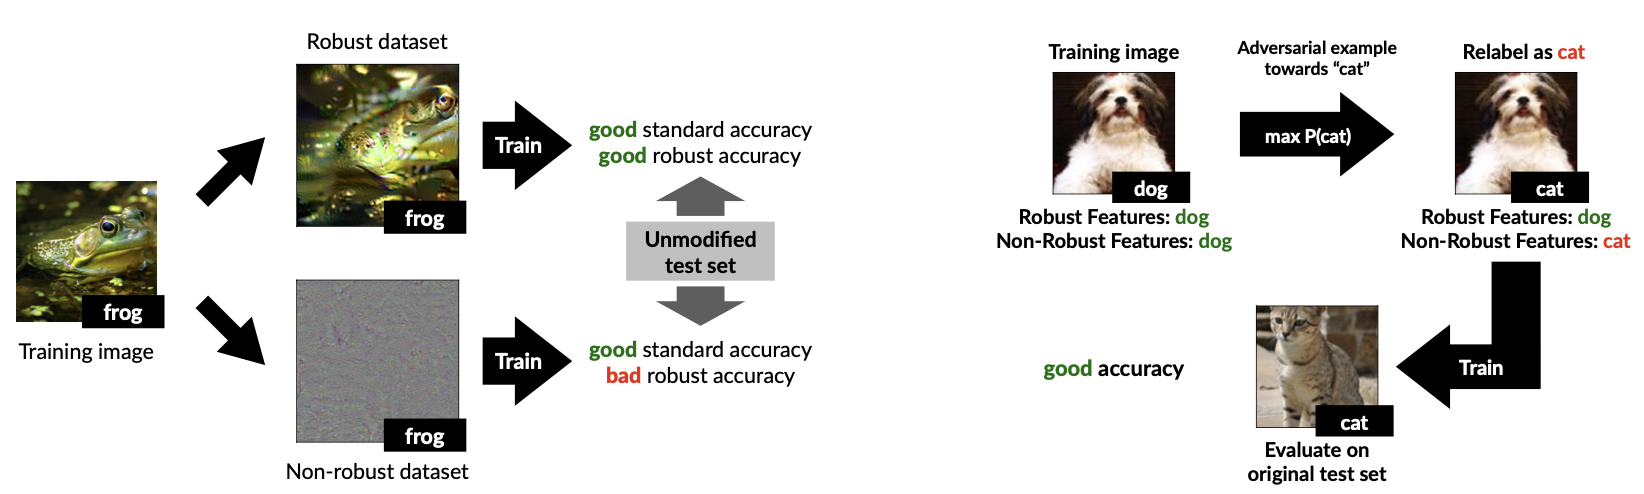
\includegraphics[width=0.8\textwidth]{assets/rml.png}
    \end{center}
\end{frame}

\begin{frame}{Non-Robust Features are also Important}
    \begin{itemize}
        \item 右图实验:通过调整Non-Robust Features 让其向某错误的标签$c_\text{wrong}$偏移,然后构建一个新的数据集,这个数据集标签是按照$c_\text{wrong}$来标记的,图像是原图像加上Non-Robust Features的偏移之后的图像。
        \item 由于 Robust Feature没有变化,人作为Robust Learner,仍然能够正确识别这些图像。
        \item 但实验结果表明,模型用这个新数据集训练,在原始test set上测试 accuracy 差不多不变,这说明模型也可以只从Non-Robust Features中学习。
    \end{itemize}
    \begin{center}
        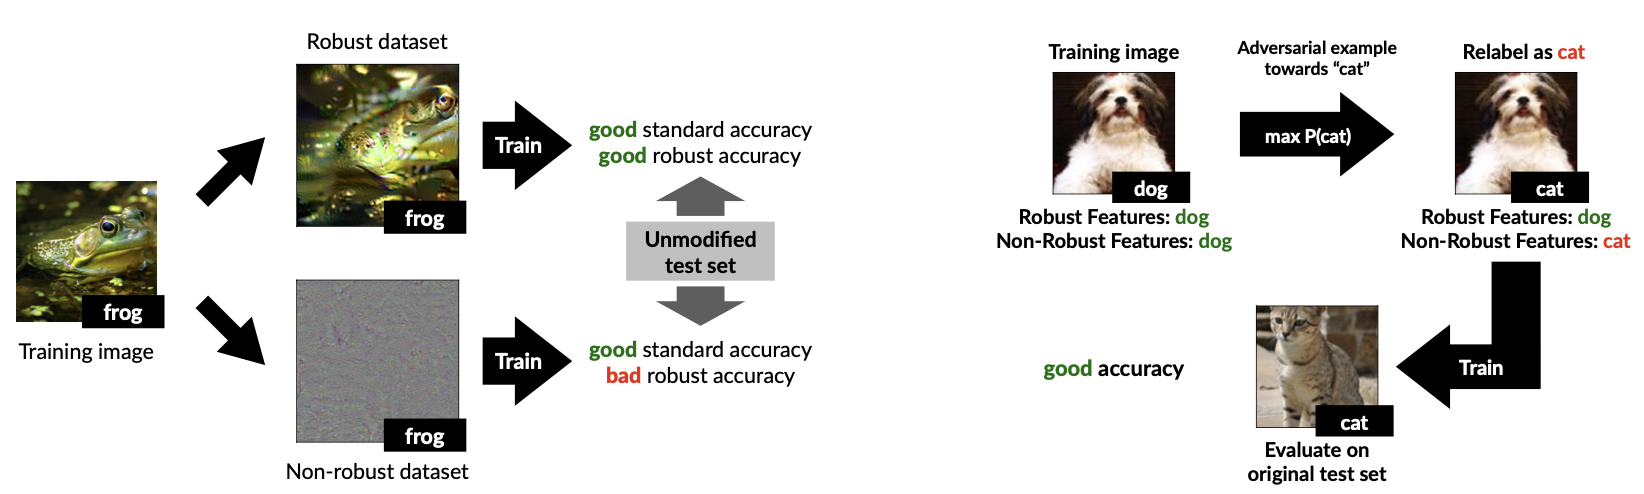
\includegraphics[width=0.8\textwidth]{assets/rml.png}
    \end{center}
\end{frame}

\begin{frame}[fragile]{Greedy Filling}
    \begin{itemize}
        \item 问题:已知一个分类器$f$,希望构建一个平滑分类器$g$,使预测更加robust。
        \item 自然想法:对单个输入$x$,不只考虑$f(x)$的值,还考虑$f(x')$的值,其中$x'$与$x$在输入空间中非常接近。
        \item 具体的:$g(x)$ 按照某概率分布函数$p(x')$(中心为$x$)加权,求不同标签$c$对应的$x'$占据的概率比例,概率比例最大的那个标签作为$g(x)$的预测结果。
        \[
            g(x) = \text{arg}\max_{c} \int_{x'} p(x') \mathbbm{1} [f(x') = c] \mathrm{d}x'
        \]
        \item Greedy Filling 算法用于计算对于给定输入点$x$和给定每个标签$c$对应的$\int_{x'} p(x') \mathbbm{1} [f(x') = c] \mathrm{d}x'$的值(即给定每种标签的概率直方图),在最坏情况下,$x$ 偏移多少就有可能让$g(x)$的预测结果发生变化。
        \item 以下为简单,只考虑二分类问题(只有两个 class $c_1$ 和 $c_2$)的Greedy Filling算法。
    \end{itemize}
\end{frame}

\begin{frame}[fragile]{Greedy Filling Example 1: Unit Ball}
    \begin{itemize}
        \item 将概率分布函数$p$取为单位球$B = \left\{x'\in \mathbb{R}^{d} | \left\| x' - x \right\| _2 \leqslant R \right\} $ 内的均匀分布
        \[
            p(x') = \begin{cases}
                \frac{1}{\text{Vol}(B)} & x' \in B \\
                0 & \text{otherwise}
            \end{cases}
        \]
        \item 目标:求$\delta$使$\left\| \delta \right\|_2 $最小,且$g(x+\delta)$能改变最大概率对应的class (二分类问题中就是两个class概率各为$50\%$)。
    \end{itemize}
\end{frame}

\begin{frame}[fragile]{Greedy Filling Example 1: Unit Ball}
    \begin{itemize}
        \item 目标:求$\delta$使$\left\| \delta \right\|_2 $最小,且$g(x+\delta)$能改变最大概率对应的class (二分类问题中就是两个class概率各为$50\%$)。
        \item 记$S_1 = \left\{ x'\in \mathbb{R}^{d} | \left\| x' - x \right\| _2 \leqslant R \right\} $, $S_2 = \left\{ x'\in \mathbb{R}^{d} | \left\| x' - x - \delta \right\| _2 \leqslant R \right\} $
        \item 不妨设$B$的体积为$1$,给定$x$点以及给定两个class $c_1$ 和 $c_2$在$x$点处概率占比为$80\%$ 和 $20\%$,按照 Greedy 的核心思想,为了让$g(x+\delta)$的预测结果发生尽量大的变化,
        \begin{itemize}
            \item 若 $\text{vol}(S_1-S_2) \geqslant 0.8$, 应将 $S_2-S_1$内全部假设为$c_2$类,由于有两个class $c_1$ 和 $c_2$在$x$点处概率占比为$80\%$ 和 $20\%$的约束,所以将 $S_1-S_2$内$0.8$体积假设为$c_1$类,其他$S_1$中体积假设为$c_2$类。
            \item 若 $\text{vol}(S_1-S_2) < 0.8$, 应将 $S_1-S_2$内全部假设为$c_1$类,$S_2-S_1$内全部为$c_2$类,$S_1 \hat S_2$ 内体积为$0.8 - \text{vol}(S_1-S_2)$ 填成 $c_1$, 其他填成 $c_2$。
        \end{itemize}
        据此可以求出$\left\| \delta \right\|_2 $的最小值。
    \end{itemize}
\end{frame}
    
\begin{frame}[fragile]{Greedy Filling Example 2: Gaussian Distribution}
    \begin{itemize}
        \item 将概率分布函数$p$取为 Gaussian Distribution
        \[
            p(x') = \frac{1}{(2\pi)^{d/2} \sigma^d} \exp\left( -\frac{1}{2\sigma^2} \left\| x' - x \right\|_2^2 \right)
        \]
        (作业中取$\sigma = 1$)
        \item 目标:求$\delta$使$\left\| \delta \right\|_2 $最小,且$g(x+\delta)$能改变最大概率对应的class。不妨假设$g(x) = c_1$。
        \item 按照 Greedy 的核心思想,为了让$g(x+\delta)$的预测结果发生尽量大的变化,应该先从 $p(x' - x - \delta)/p(x' - x)$ 最大的 $x'$ 处开始设成 $c_2$,因为先从这里开始选取 $c_2$ 可以让$g(x+\delta)$中$c_2$的成分相较$g(x)$中$c_2$的成分增加最多。
        \item 再由高斯分布的特性,$p(x' - x - \delta)/p(x' - x)$ 的等值线是超平面,退化为一维问题,$\left\| \delta \right\|_2 $的最小值容易求解。(剩下的步骤参考习题课)
    \end{itemize}
\end{frame}


\begin{frame}[fragile]{Greedy Filling}
    \begin{itemize}
        \item 问题:已知一个分类器$f$,希望构建一个平滑分类器$g$,使预测更加robust。
        \item 自然想法:对单个输入$x$,不只考虑$f(x)$的值,还考虑$f(x')$的值,其中$x'$与$x$在输入空间中非常接近。
        \item 具体的:$g(x)$ 按照某概率分布函数$p(x')$(中心为$x$)加权,求不同标签$c$对应的$x'$占据的概率比例,概率比例最大的那个标签作为$g(x)$的预测结果。
        \[
            g(x) = \text{arg}\max_{c} \int_{x'} p(x') \mathbbm{1} [f(x') = c] \mathrm{d}x'
        \]
        \item Greedy Filling 算法用于计算对于给定输入点$x$和给定每个标签$c$对应的$\int_{x'} p(x') \mathbbm{1} [f(x') = c] \mathrm{d}x'$的值(即给定每种标签的概率直方图),在最坏情况下,$x$ 偏移多少就有可能让$g(x)$的预测结果发生变化。
        \item 以下为简单,只考虑二分类问题(只有两个 class $c_1$ 和 $c_2$)的Greedy Filling算法。
    \end{itemize}
\end{frame}

\begin{frame}[fragile]{Greedy Filling Example 1: Unit Ball}
    \begin{itemize}
        \item 将概率分布函数$p$取为单位球$B = \left\{x'\in \mathbb{R}^{d} | \left\| x' - x \right\| _2 \leqslant R \right\} $ 内的均匀分布
        \[
            p(x') = \begin{cases}
                \frac{1}{\text{Vol}(B)} & x' \in B \\
                0 & \text{otherwise}
            \end{cases}
        \]
        \item 目标:求$\delta$使$\left\| \delta \right\|_2 $最小,且$g(x+\delta)$能改变最大概率对应的class (二分类问题中就是两个class概率各为$50\%$)。
    \end{itemize}
\end{frame}

\begin{frame}[fragile]{Greedy Filling Example 1: Unit Ball}
    \begin{itemize}
        \item 目标:求$\delta$使$\left\| \delta \right\|_2 $最小,且$g(x+\delta)$能改变最大概率对应的class (二分类问题中就是两个class概率各为$50\%$)。
        \item 记$S_1 = \left\{ x'\in \mathbb{R}^{d} | \left\| x' - x \right\| _2 \leqslant R \right\} $, $S_2 = \left\{ x'\in \mathbb{R}^{d} | \left\| x' - x - \delta \right\| _2 \leqslant R \right\} $
        \item 不妨设$B$的体积为$1$,给定$x$点以及给定两个class $c_1$ 和 $c_2$在$x$点处概率占比为$80\%$ 和 $20\%$,按照 Greedy 的核心思想,为了让$g(x+\delta)$的预测结果发生尽量大的变化,
        \begin{itemize}
            \item 若 $\text{vol}(S_1-S_2) \geqslant 0.8$, 应将 $S_2-S_1$内全部假设为$c_2$类,由于有两个class $c_1$ 和 $c_2$在$x$点处概率占比为$80\%$ 和 $20\%$的约束,所以将 $S_1-S_2$内$0.8$体积假设为$c_1$类,其他$S_1$中体积假设为$c_2$类。
            \item 若 $\text{vol}(S_1-S_2) < 0.8$, 应将 $S_1-S_2$内全部假设为$c_1$类,$S_2-S_1$内全部为$c_2$类,$S_1 \hat S_2$ 内体积为$0.8 - \text{vol}(S_1-S_2)$ 填成 $c_1$, 其他填成 $c_2$。
        \end{itemize}
        据此可以求出$\left\| \delta \right\|_2 $的最小值。
    \end{itemize}
\end{frame}
    
\begin{frame}[fragile]{Greedy Filling Example 2: Gaussian Distribution}
    \begin{itemize}
        \item 将概率分布函数$p$取为 Gaussian Distribution
        \[
            p(x') = \frac{1}{(2\pi)^{d/2} \sigma^d} \exp\left( -\frac{1}{2\sigma^2} \left\| x' - x \right\|_2^2 \right)
        \]
        (作业中取$\sigma = 1$)
        \item 目标:求$\delta$使$\left\| \delta \right\|_2 $最小,且$g(x+\delta)$能改变最大概率对应的class。不妨假设$g(x) = c_1$。
        \item 按照 Greedy 的核心思想,为了让$g(x+\delta)$的预测结果发生尽量大的变化,应该先从 $p(x' - x - \delta)/p(x' - x)$ 最大的 $x'$ 处开始设成 $c_2$,因为先从这里开始选取 $c_2$ 可以让$g(x+\delta)$中$c_2$的成分相较$g(x)$中$c_2$的成分增加最多。
        \item 再由高斯分布的特性,$p(x' - x - \delta)/p(x' - x)$ 的等值线是超平面,退化为一维问题,$\left\| \delta \right\|_2 $的最小值容易求解。(剩下的步骤参考习题课)
    \end{itemize}
\end{frame}

\section{Hyperparameter Optimization}


\section{Interpretability}

\begin{frame}{Interpretability}
    思想:如果给模型一个输入,模型直接输出一个结果,模型对用户来说是一个黑箱,这对一些场景下是不合适的。希望模型能够输出一些直观解释,让用户能理解模型的决策过程。

    几种方法:
    \begin{itemize}
        \item LIME Algorithm
        \item Integrated Method
        \item SHAP
    \end{itemize}
\end{frame}

\begin{frame}{LIME}
    一般框架:
    \begin{itemize}
        \item 设希望被解释的模型为 $f: \mathbb{R}^{d}\to \mathbb{R}$,输入为 $x$。目标:解释为什么 $f(x)$ 这样输出。
        \item 设 $g \in G$ 是一个解释模型,定义域为 $\left\{ 0, 1 \right\}^{d'} $代表 $x$可解释的表示的二进制向量。
        \item $\Omega(g)$代表解释的复杂度度量。
        \item $\Pi_x(z)$ 表示 instance $z$ 与 $x$ 的接近程度。
        \item 目标:最小化 $\xi(x) = \text{arg}\min_{g \in G}\left( L(f, g, \Pi_x) + \Omega(g) \right) $,$\xi(x)$ 就是最优解释。
    \end{itemize}
    我们只考虑 $G$ 是线性模型族的情况,即 $g(z') = w_g \cdot z'$。
    
    通常取 $L(f, g, \Pi_x) = \prod_{z, z' \in Z} \Pi_x (z) \cdot (f(z) - g(z'))^{2}$,其中$\Pi_x(z) = \exp\left( - D(x, z)^{2} / \sigma^{2} \right) $,$\Omega(g) = \infty \mathbbm 1[\left\| w_g \right\| _0 > k]$

\end{frame}

\begin{frame}{LIME Algorithm}
    算法:
    \begin{center}
        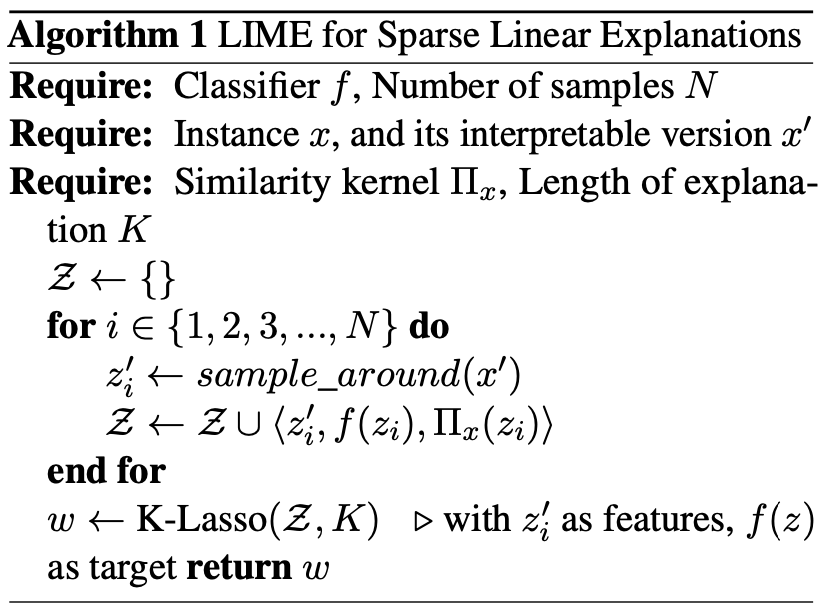
\includegraphics[width=0.6\textwidth]{assets/lime.png}
    \end{center}
\end{frame}

\begin{frame}{LIME Algorithm}
\begin{itemize}
    \item 在图像分类模型解释问题中,每个可解释的$z$是对每个super-pixel分配0或1。
    \item 为了解释为什么模型将一个弹着吉他的狗头人识别出来是Labrador、Electric guitar和Acoustic guitar,按照上述算法中$K-Lasso$ 的原理,最终每种标签对应的返回权重$w$是比较稀疏的,将这些非$0$的$w$分量对应的super-pixel按原图输出出来,$0$的$w$分量对应的super-pixel输出灰色图像,可得到下图。
\end{itemize}
\begin{center}
    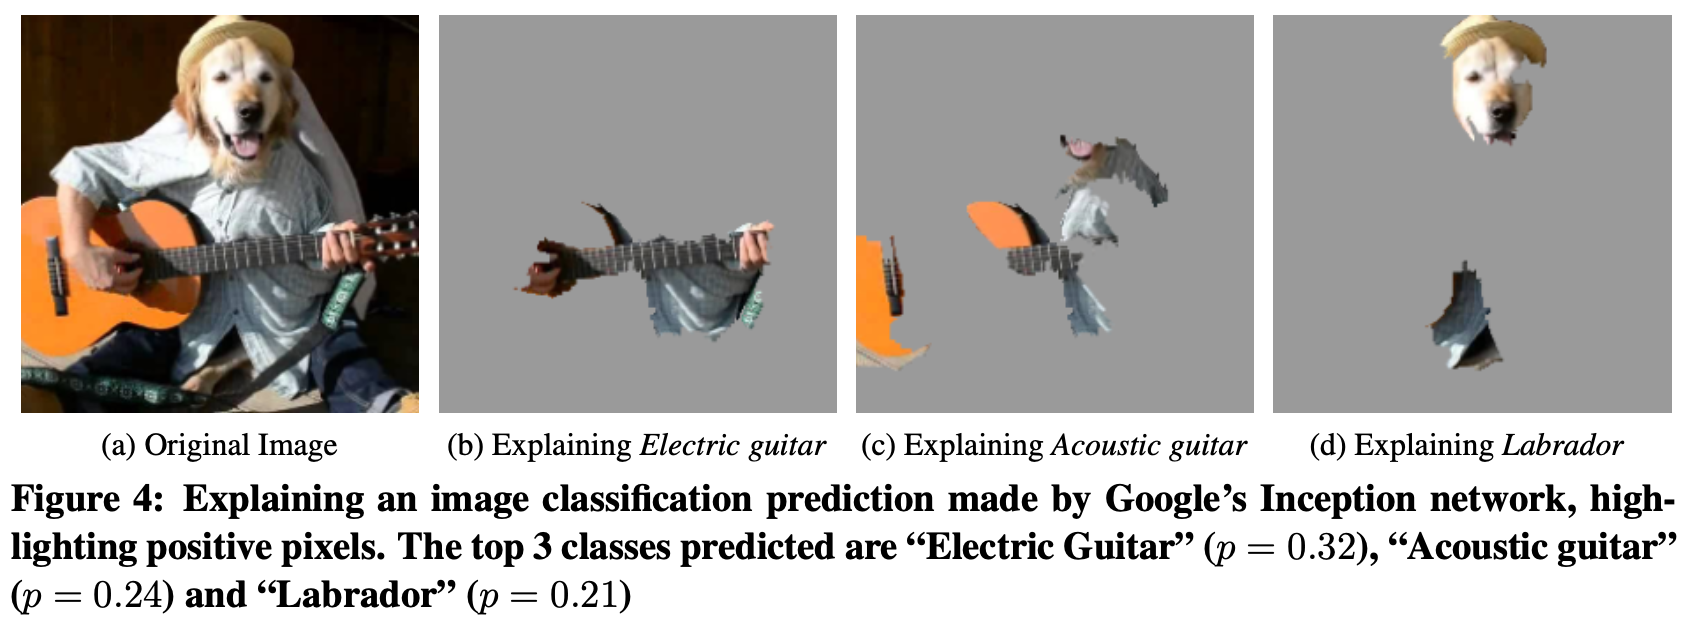
\includegraphics[width=0.75\textwidth]{assets/limee.png}
\end{center}
\end{frame}

\begin{frame}{Integrated Method}
    思想:Integrated Method论文中指出了一些关于可解释性的公理,然后从这些公理出发推导可能的解释方法。Integrated Gradients满足所有他们提出的公理。

    \begin{itemize}
        \item 设函数 $F: \mathbb{R}^{n} \to [0, 1]$ 表示一个 deep network,$x\in \mathbb{R}^{n}$ 是输入,$x'\in \mathbb{R}^{n}$ 是一个 baseline input。
        \item 定义 
        \[
        \text{IntegratedGrads}_i(x) := (x_i - x'_i) \cdot \int_{\alpha=0}^{1} \frac{\partial F(x' + \alpha(x - x'))}{\partial x_i}  \mathrm{d}\alpha  
        \]
        \item Completeness: 
        \[
        \sum_{i=1}^{n}\text{IntegratedGrads}_i(x) = F(x) - F(x')
        \]
        证明方法:简单的微积分。
    \end{itemize}
\end{frame}

\begin{frame}{Shapley Value Algorithm (a.k.a. SHAP)}
    \begin{itemize}
        \item 问题:$x_1, x_2, \cdots, x_n$ 是输入变量,$S \subseteq \left\{ x_1, x_2, \cdots, x_n \right\} $, $f(S)$ 表示 $S$ 对最终结果的贡献。如何计算每个输入变量单独的作用?
        \item 生动的例子:抢银行分钱,总钱数为 $f([n])$.
        \item $x_i$ 的作用是($x_i$应该分得的钱)
    \[
        \phi_i(f) = \sum_{S \subseteq [n]\backslash \left\{ i \right\}} \frac{\left| S \right| ! \left( n - |S| - 1 \right) !}{n!} \Big( f(S \cup \left\{ i \right\}) - f(S) \Big)
    \]
    \item 性质:
    \[
        \sum_{i=1}^{n} \phi_i(f) = f([n])  
    \]
    \end{itemize}
\end{frame}

\section{Rectified Flow}

\begin{frame}{Rectified Flow}
    算法:
    \begin{center}
        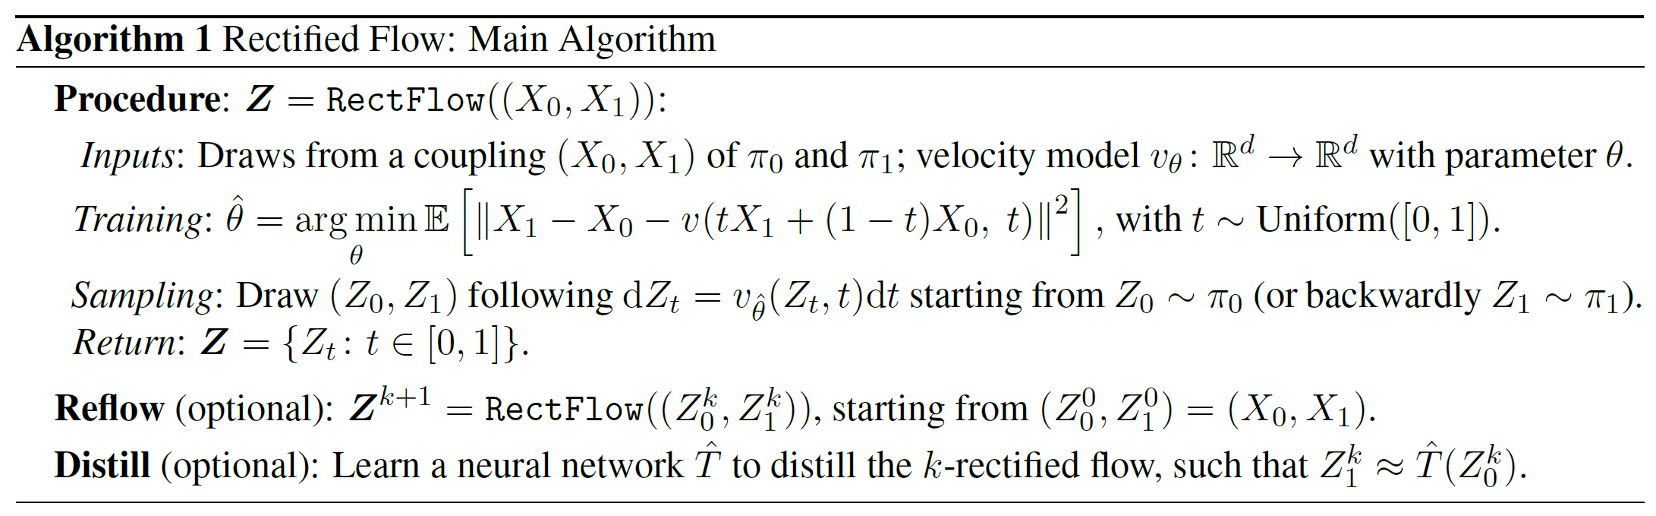
\includegraphics[width=0.8\textwidth]{assets/rf.png}
    \end{center}
\end{frame}
\section{RoPE}

\begin{frame}{Transformer}
    \begin{itemize}
        \item 记 $S_N = \left\{ w_i \right\}_{i=1}^{N} $ 是$N$个输入词汇序列
        \item $E_N=\left\{ x_i \right\}_{i=1}^{N}$ 是对应的 word embedding, $x_i$中没有位置信息
        \item 融入位置信息:
        \[
            \begin{cases} q_m &= f_q(x_m, m) \\ k_n &= f_k(x_n, n) \\ q_n &= f_v(x_n, n) \end{cases}
        \]
        \item attention weight: $a_{mn} = \frac{\exp(q_m^{T}k_n / \sqrt d)}{ \sum_{j=1}^{N}\exp(q_m^{T}k_j / \sqrt d)}$
        \item output embedding: $o_m = \sum_{n=1}^{N} a_{mn} v_n$
    \end{itemize}
\end{frame}

\begin{frame}{Rotary Position Embedding (a.k.a. RoPE)}
    \begin{itemize}
        \item 在 Transformer 模型中,RoPE 是一种将token位置融入 attention 模块的方法。
        \item 核心思想:希望计算 attention weight 的时候 $q_m^{T} k_n$ 点积结果只与 $x_m, x_n$ 和 $m-n$ 相关。
        \item 2D 情况下,一个解为复数解,可以等价地写成矩阵形式方便计算。
        \begin{center}
            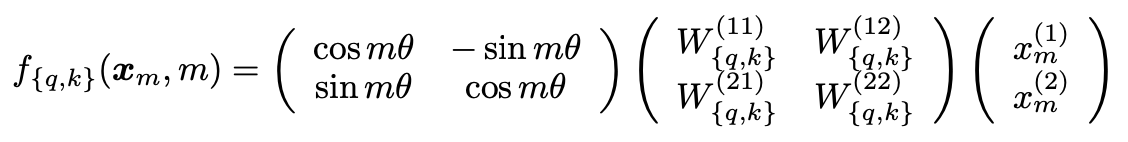
\includegraphics[width=0.6\textwidth]{assets/rope2.png}
        \end{center}
        \item 更高维情况下可以写成
        \begin{center}
            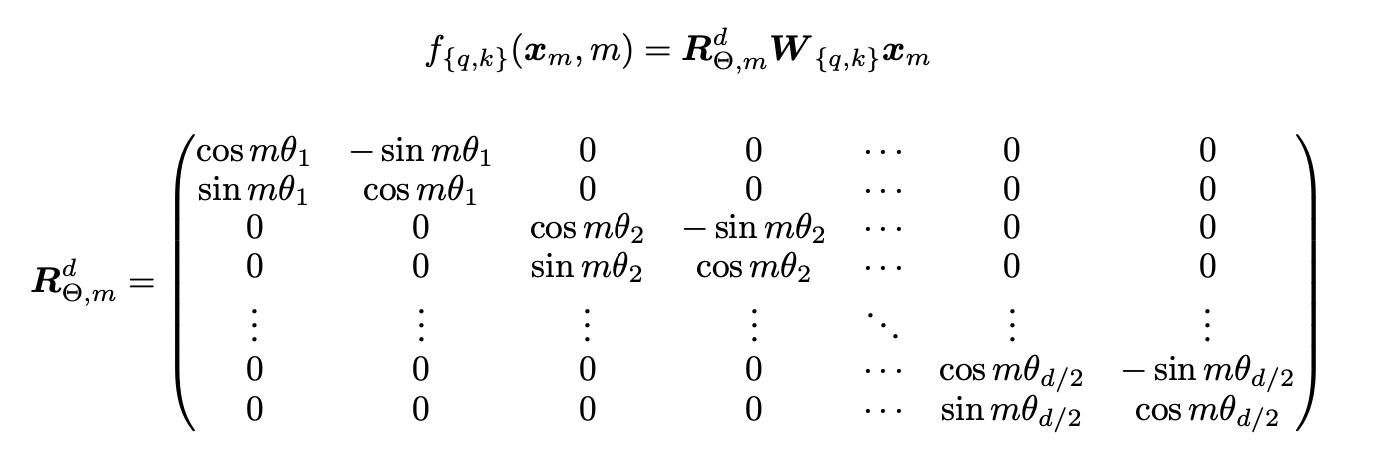
\includegraphics[width=0.5\textwidth]{assets/roped.png}
        \end{center}
        其中 $\Theta = \left\{ \theta_i = 10000^{-2(i-1)/d}, i \in [1, 2, \cdots, d / 2] \right\} $
    \end{itemize}
\end{frame}


\begin{frame}[fragile]{}
\framesubtitle{}
\end{frame}

\section{Personalization}

\begin{frame}[fragile]{Adding images}
\begin{columns}
\begin{column}{0.7\textwidth}

\end{column}
\begin{column}{0.3\textwidth}

\includegraphics[width=\textwidth]
{assets/logo_RGB}
\end{column}
\end{columns}
\end{frame}

\section{Summary}


\backmatter
\end{document}